% BACKUP: This content was removed from case-study.tex
% Section: Motivation: Analyzing eBPF Kernel Features with Data Analysis

\subsection{Motivation: Analyzing eBPF Kernel Features with Data Analysis}

To understand the limitations of traditional data analysis methods, we begin by analyzing the evolution of eBPF kernel features using well-defined kernel commits. Traditional methods allow us to study the development of various eBPF features, such as helpers, maps, attach types, and other functionalities. We obtained feature pairs from eBPF documentation~\cite{ebpfdocs} and combined them with Git commit data.

\subsubsection{How Do All eBPF Features Evolve Over Time?}

Figure~\ref{fig:cumulative_feature_timeline} shows trends in the adoption of new features within the overall eBPF subsystem. Helpers and kfuncs exhibit the most significant growth, supporting various use cases and changes, while other features have shown steady increases over the past four years, indicating their maturation.

\begin{figure}[ht]
    \centering
    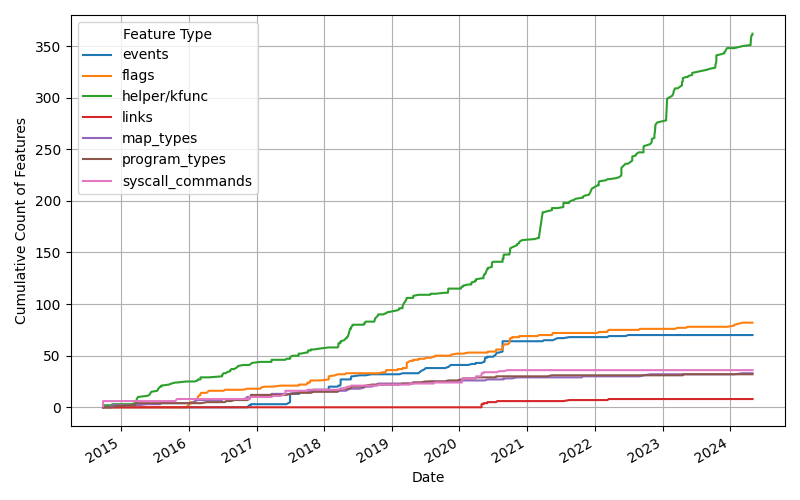
\includegraphics[width=\linewidth]{feature-analysis/cumulative_bpf_features_timeline.png}
    \caption{Cumulative eBPF Features Timeline}
    \label{fig:cumulative_feature_timeline}
\end{figure}

\subsubsection{Timeline of eBPF Helper Functions vs.\ Kfuncs}

Figure~\ref{fig:cumulative_helper_kfunc_timeline} illustrates the evolution of eBPF helper functions and kfuncs over time. Since 2023, helper functions have remained stable with almost no new additions, whereas kfuncs are growing rapidly; this demonstrates the community's interest in expanding kernel interaction via kfuncs, and all new use cases now tend to use kfuncs to influence kernel behavior, signaling a shift toward deeper kernel integrations.

\begin{figure}[ht]
    \centering
    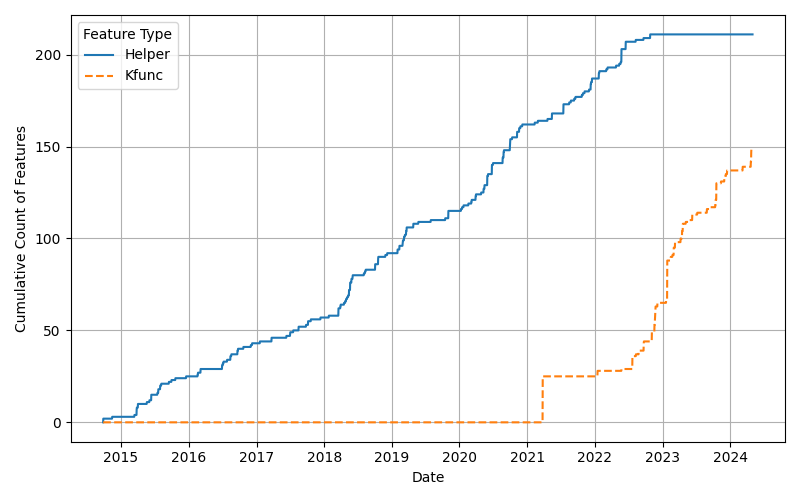
\includegraphics[width=\linewidth]{feature-analysis/cumulative_helper_kfunc_timeline.png}
    \caption{Cumulative Helper and kfunc Timeline}
    \label{fig:cumulative_helper_kfunc_timeline}
\end{figure}

\subsubsection{What Are the Patterns in Other eBPF Features?}

Figure~\ref{fig:cumulative_without_helper_timeline} examines the evolution of eBPF features, excluding helpers and kfuncs, with a focus on core eBPF functionalities and their impact on the overall subsystem. After 2020, core features such as events, flags, map types, and program types have stabilized. Notably, the introduction of \textbf{bpf\_link} coincides with the effort on the management of growing use cases and complexity, resulting in a significant difference observed before and after its introduction.


\begin{figure}[ht]
    \centering
    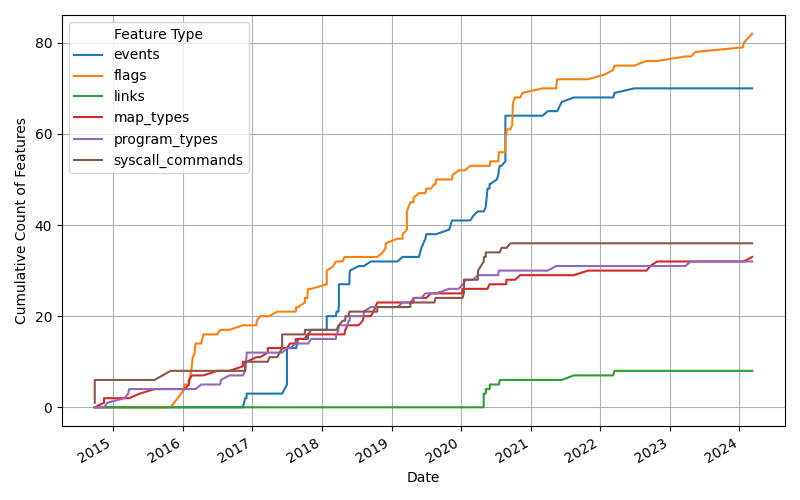
\includegraphics[width=\linewidth]{feature-analysis/cumulative_bpf_features_timeline_no_helper_kfunc.png}
    \caption{Cumulative eBPF Features Timeline Without Helpers and kfuncs}
    \label{fig:cumulative_without_helper_timeline}
\end{figure}

\paragraph{However\ldots}

The analysis of eBPF features mainly relies on kernel structured definitions and data sources obtained by humans, which is limited by data availability and the time-consuming process of manual data collection.

There is a massive amount of unstructured data in the form of commit messages, code changes, and developer discussions that can provide valuable insights into the evolution and design decisions of eBPF features. While it is possible for humans to perform empirical analysis on some of this data, covering all of it is practically \emph{impossible}.

\textbf{Can AI assist us?} Instead of relying on large language models (LLMs) to attempt kernel coding—which may yield incorrect answers—we propose a different quantitative approach.

By carefully designing a \emph{survey} and utilizing LLMs to \emph{transform} unstructured data like commits and emails into well-organized, structured, and easy-to-analyze datasets, we can perform \textbf{quantitative} analysis using traditional methods. In this way, AI can help analyze data and provide answers quickly; this capability is already a feature of platforms like ChatGPT.